\textbf{Цели работы:} изучение поляризации света при отражении и преломлении; нахождение степени поляризации лазерного излучения.

\textbf{Приборы и принадлежности:} экспериментальная установка для изучения поляризации света, представляющая собой модульный учебный комплекс по волновой оптике (МУК-ОВ).

Установка состоит из механического и электронного блоков (рис. 4.8). Механический блок 1 представляет собой основание 10, на котором установлены и закреплены: стойка 17, служащая вертикальной оптической скамьей; турель 19; защитный экран 18; электронный блок 5. На стойке смонтированы оптические узлы 2--4, 16, которые могут вращаться и выводиться из поля зрения, если при выполнении эксперимента они не используются. Защитный экран 18 не вращается и участвует во всех экспериментах на данной установке.

Электронный блок 5 содержит кнопки, индикаторы измерительных устройств и окна фотоприемников.

При выполнении данной лабораторной работы используются следующие узлы механического блока 1: защитный экран 18, поляризатор 2, устройство для измерения угла Брюстера 4 с матовой полупрозрачной шкалой, анализатор 16. Вращающаяся втулка на устройстве 4 позволяет изменять угол падения луча на стеклянную пластинку относительно вертикальной шкалы. Поляризатор 2 и анализатор 16 снабжены угломерной шкалой. На электронном блоке 5 используются: кнопка включения лазера 12; регулятор интенсивности 13; кнопка переключения фотоприемников 8; индикатор относительной интенсивности света 7; четыре индикатора включенного фотоприемника 14 с определенным диапазоном длин волн; кнопка включения электронного блока «Сеть» 9 и окно фотоприемника лазерного излучения 6.

\begin{figure}[H]
    \def\thefigure{4.8}
    \protect\phantomsection 
	
    \centering
	\captionsetup{justification=centering}
    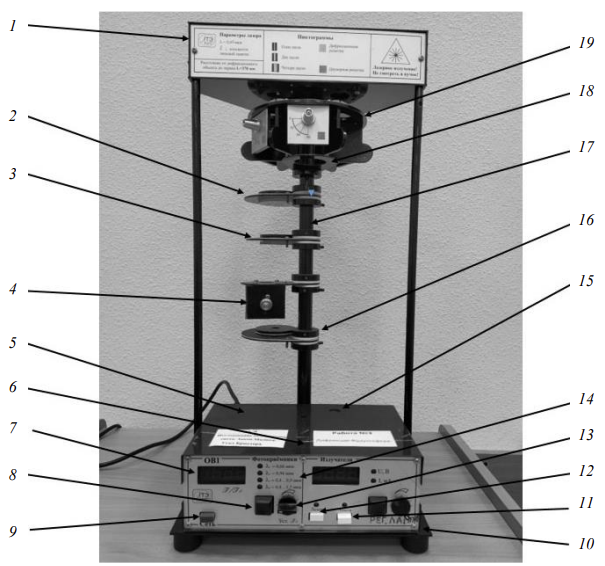
\includegraphics[width=0.8\linewidth]{figs/1.png}
	\caption{Экспериментальная установка по волновой оптике (МУК-ОВ)}
	\label{fig:exp_setup}
\end{figure}

В лабораторной установке на индикаторе 7 показывается не абсолютная, а относительная интенсивность излучения $I_{\text{отн}} = I/I_0$, где $I_0$ -- некоторая константа, задаваемая чувствительностью измерительного прибора.

\newpage
\centeredsection{\MakeUppercase{Исследуемые закономерности}}
В данной работе проводится проверка закона Малюса, определяется степень поляризации лазерного излучения и находится показатель преломления стекла через угол Брюстера.

\subsection*{1. Проверка закона Малюса и определение степени поляризации}

\subsubsection*{Теоретическая основа:}
Интенсивность $I$ плоскополяризованного света, прошедшего через анализатор, зависит от угла $\varphi$ между плоскостью поляризации света и плоскостью пропускания анализатора согласно закону Малюса:
\[ I(\varphi) = I_{max} \cdot \cos^2{\varphi} \]
где $I_{max}$ --- максимальная интенсивность света, прошедшего через анализатор.

Степень поляризации $P$ для частично поляризованного света определяется по формуле:
\[ P = \frac{I_{max} - I_{min}}{I_{max} + I_{min}} \]
где $I_{min}$ --- минимальная интенсивность.

\subsubsection*{Порядок действий и обработка:}
\begin{enumerate}
    \item \textbf{Снятие данных для закона Малюса:} Пропустив луч лазера через поляризатор и анализатор, измерьте зависимость относительной интенсивности $I_\text{отн}$ от угла поворота анализатора $\varphi$ с шагом в 10$^\circ$.
    
    \item \textbf{Обработка:} Постройте на миллиметровой бумаге экспериментальный график зависимости нормированной интенсивности $I_\text{отн}(\varphi)/I_{\text{отн}, max}$ от угла $\varphi$. Сравните его с теоретической зависимостью $y = \cos^2{\varphi}$, построенной на том же графике.
    
    \item \textbf{Определение степени поляризации:} Найдите максимальное ($I_{\text{отн}, max}$) и минимальное ($I_{\text{отн}, min}$) значения интенсивности, вращая анализатор. Рассчитайте степень поляризации $P$ по приведённой выше формуле.
\end{enumerate}

\subsection*{2. Определение угла Брюстера и показателя преломления}

\subsubsection*{Теоретическая основа:}
При падении света на границу раздела двух диэлектриков под \textbf{углом Брюстера} $\theta_Б$ отраженный луч становится полностью плоскополяризованным, а его интенсивность --- минимальной. Угол Брюстера связан с показателем преломления $n$ вещества \textbf{законом Брюстера}:
\[ \tan(\theta_\text{Б}) = n \]

\subsubsection*{Порядок действий и обработка:}
\begin{enumerate}
    \item \textbf{Измерение:} На пути лазерного луча установите стеклянную пластину на поворотном устройстве. Изменяя угол падения луча $\theta$, визуально найдите такое его значение, при котором интенсивность отраженного луча будет минимальной.
    
    \item \textbf{Обработка:} Измеренный угол падения, при котором наблюдается минимум интенсивности, является углом Брюстера $\theta_\text{Б}$. Вычислите показатель преломления $n$ материала пластины по формуле $n = \tan(\theta_\text{Б})$.
\end{enumerate}



















\newpage
\centeredsection{\MakeUppercase{Указания по проведению эксперимента}}

\textbf{1. Нахождение степени поляризации излучения лазера.}
\begin{enumerate}
    \item[1.1.] Включить лазерный источник света, соблюдая правила техники безопасности (не допускать прямого попадания лазерного излучения в глаз). Турель 19 (рис. 4.8) установить так, чтобы излучение от источника проходило ее беспрепятственно.
    \item[1.2.] Кнопкой переключения фотоприемников 8 установить диапазон длин волн $\lambda_4 = 0.4...1.2$ мкм, о чем будет свидетельствовать включение одного из индикаторов 14. Вращением ручки 13 добиться наибольших показаний максимальной относительной интенсивности $I_{\text{отн}} = I/I_0$ на индикаторе 7 (рис. 4.8).
    \item[1.3.] Поскольку выходящий из лазерного источника свет является эллиптически-поляризованным, то для превращения его в плоскополяризованный на пути лазерного луча поместить поляризатор 2. Стрелку шкалы поляризатора установить на $0^\circ$.
    \item[1.4.] Установить между лазером и фотоприемником анализатор 16.
    \item[1.5.] Вращая анализатор и непрерывно следя за показаниями цифрового индикатора интенсивности, измерить максимальное ($I_{\text{отн}\ max}$) и минимальное ($I_{\text{отн}\ min}$) значения относительной интенсивности проходящего излучения. Наблюдения выполнить 5 раз и результаты записать в протокол.
\end{enumerate}

\textbf{2. Проверка закона Малюса.}
\begin{enumerate}
    \item[2.1.] Схема установки (рис. 4.8) для проверки закона Малюса состоит из источника света -- лазера, поляризатора 2, анализатора 16, фотоприемника 6. Правила включения лазерного источника и настройки установки не меняются и соответствуют пп. 1.1--1.4.
    \item[2.2.] Вращая анализатор, снять зависимость относительной интенсивности $I_\text{отн}(\varphi)$ от угла поворота анализатора $\varphi$ через каждые $10^\circ$ от $\varphi = -150^\circ$ до $\varphi = +150^\circ$, проходя через $0^\circ$ (вращать против часовой стрелки). Результаты наблюдений занести в протокол.
\end{enumerate}

\textbf{3. Нахождение угла Брюстера для стеклянной пластинки.}
\begin{enumerate}
    \item[3.1.] Схема установки (см. рис. 4.8) по определению угла Брюстера для стеклянной пластинки состоит из источника света -- лазера, поляризатора 2, устройства для измерения угла Брюстера 4 с матовой полупрозрачной вертикальной шкалой и фотоприемника 6. В данном эксперименте анализатор 16 не используется, поэтому его нужно установить в положение вне хода лазерного луча. Правила включения лазерного источника и настройки установки не меняются и соответствуют пп. 1.1--1.3.
    \item[3.2.] Установить по ходу луча устройство для измерения угла Брюстера 4.
    \item[3.3.] Вращая втулку на устройстве 4, визуально пронаблюдать за изменениями интенсивности луча лазера, отраженного от стеклянной пластинки под углом $\theta$, фиксируемым на вертикальной шкале.
    \item[3.4.] Добиться минимальной интенсивности луча, визуально наблюдаемого при отражении от стеклянной пластинки, что соответствует падению светового луча на стеклянную пластинку под углом Брюстера. Определить по шкале числовое значение полученного угла $\theta_Б$. Результат наблюдений занести в протокол.
    \item[3.5.] Выключить установку кнопкой «Сеть» 9.
\end{enumerate}




















\newpage
\thispagestyle{empty}
\centeredsection{ПРОТОКОЛ НАБЛЮДЕНИЙ}

\begin{table}[H]
    \centering
    \caption{Измерение максимальной и минимальной интенсивности ($\theta_I=0,01$)}
    \label{tab:polarization}
    \begin{tabularx}{\linewidth}{|c|C|C||C|C|}
        \hline
            \multirow{2}{*}{№} & \multicolumn{2}{c||}{Излучение лазера} & \multicolumn{2}{c|}{Преломлённый свет}  \\
        \cline{2-5}
            &
            \textbf{$I_{max}$} & \textbf{$I_{min}$} & \textbf{$I_{max}$} & \textbf{$I_{min}$} \\
        \hline
            1 & & & & \\
        \hline
            2 & & & & \\
        \hline
            3 & & & & \\
        \hline
    \end{tabularx}
\end{table}

\begin{table}[H]
    \centering
    \caption{Зависимость интенсивности от угла анализатора}
    \label{tab:malus_law_corrected}
    \begin{tabularx}{\linewidth}{|c|c|C||c|c|C|}
        \hline
        \textbf{$\varphi$, $^{\circ}$} & \textbf{$\cos^2\varphi$} & \textbf{$I_\varphi \cdot 10^3$} & \textbf{$\varphi$, $^{\circ}$} & \textbf{$\cos^2\varphi$} & \textbf{$I_\varphi \cdot 10^3$} \\
        \hline
        0 & 1.000 & & 80 & 0.030 & \\
        \hline
        10 & 0.970 & & 90 & 0.000 & \\
        \hline
        20 & 0.883 & & 100 & 0.030 & \\
        \hline
        30 & 0.750 & & 110 & 0.117 & \\
        \hline
        40 & 0.587 & & 120 & 0.250 & \\
        \hline
        50 & 0.413 & & 130 & 0.413 & \\
        \hline
        60 & 0.250 & & 140 & 0.587 & \\
        \hline
        70 & 0.117 & & 150 & 0.750 & \\
        \hline
    \end{tabularx}
\end{table}

\vfill
\noindent
Рахметов А. Р., гр. 4494 ~~\hrulefill~~ «\rule{1cm}{0.4pt}» \rule{3cm}{0.4pt} 20\rule{0.75cm}{0.4pt} г.

% \newpage
% \centeredsection{Вопросы}
% \section*{Вопрос 1 (№19).}
% \begin{quote}
%     \textit{Сформулируйте принцип суперпозиции волн.}
% \end{quote}

% Принцип суперпозиции утверждает, что если в среде одновременно распространяется несколько волн, то результирующее смещение среды в любой точке и в любой момент времени равно векторной сумме смещений, которые создавала бы каждая из волн в отдельности.

% \begin{equation*}
%     \vec{E} = \sum_{i=1}^{n} \vec{E}_i
% \end{equation*}



% \section*{Вопрос 2 (№37).}
% \begin{quote}
%     \textit{Какова интерференция при отражении света от плоскопараллельной пластинки? Покажите ход лучей. Рассчитайте оптическую разность хода.}
% \end{quote}
% \begin{figure}[H]
%     \centering
%     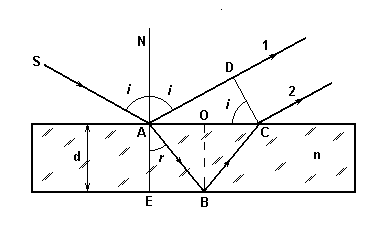
\includegraphics[width=0.5\linewidth]{interferenc.png}
% \end{figure}
% Лучи (1) и (2) являются когерентными (т.е. колебания происходят синхронно; т.к. они произошли от одного исходного луча) и распространяются параллельно друг другу. Их интерференция наблюдается в плоскости, перпендикулярной лучам (1) и (2).

% Оптическая разность хода (разность хода; $\Delta$) --- это разница между оптическими длинами путей, пройденных двумя когерентными световыми волнами от общего источника до одной и той же точки: $\Delta = l_2-l_1=l_1-l_2$; $\Delta = m\lambda$ (для max); $\Delta = (m+\frac12)\lambda$ (для min), где $l_\text{опт}=n\cdot l_\text{геом}$.

% Оптическая длина пути --- расстояние, на которое свет распространился бы в вакууме за время его прохождения между данными двумя точками.

% Для примера выше оптическая разность хода будет равна: $\Delta=2nd\cos(i')+\frac{\lambda}2$.

% \newpage
% \centeredsection{ИДЗ №33}
% \begin{quote}
%     Пучок монохроматических ($\lambda= 600$ нм) световых волн падает под углом $\alpha= 30^\circ$ на находящуюся в воздухе мыльную плёнку ($n = 1,30$). При какой наименьшей толщине $d$ плёнки отражённые световые волны будут: 1) максимально ослаблены интерференцией; 2) максимально  усилены?
% \end{quote}
% \begin{figure}[H]
%     \centering
%     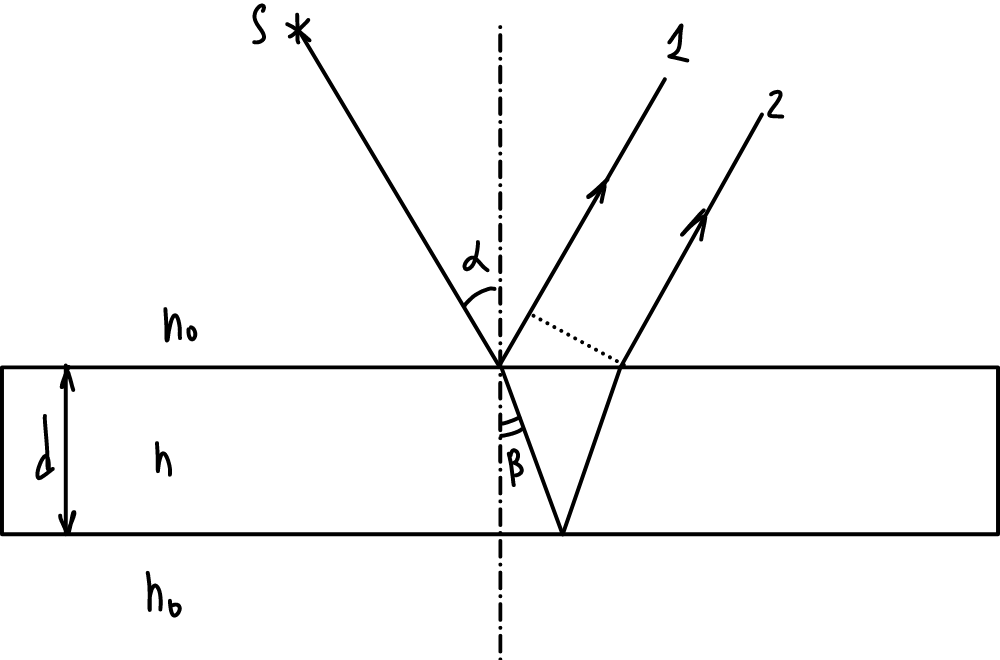
\includegraphics[width=0.5\linewidth]{IMG_20250928_220659_551.jpg}
% \end{figure}

% \begin{enumerate}
%     \item Рассчитаем $\cos\beta$
%         $$n_0\sin\alpha=n\sin\beta\Rightarrow\sin\beta=\frac{n_0\sin\alpha}{n}=\frac{1\cdot\sin(30^\circ)}{1,3}=\frac{5}{13}$$

%         $$\cos\beta=\sqrt{1-\sin^2\beta}=\sqrt{\frac{144}{169}}=\frac{12}{13}$$

%         $$\cos\beta=\frac{12}{13}$$

%     \item Найдем разность хода
%         $$l_1=\frac\lambda2;\qquad l_2=2nd\cos\beta;\qquad \Delta=l_2-l_1$$
%         $$\Delta=2nd\cos\beta-\frac{\lambda}{2}$$
%     \item Максимальное ослабление ($\Delta=(m+\frac12)\lambda$)
%         $$2nd\cos\beta-\frac{\lambda}{2} = (m+\frac12)\lambda$$
%         $$2nd\cos\beta = (m+\frac12)\lambda + \frac{\lambda}{2}$$
%         $$2nd\cos\beta = (m+1)\lambda, m\in\mathbb{Z} \Rightarrow m+1\equiv m$$
%         $$2nd\cos\beta = m\lambda$$
%         $$d = \frac{m\lambda}{2n\cos\beta},~~d_{min}\text{ при } m=1$$
%         $$d = \frac{\lambda}{2n\cos\beta}$$
%         $$d_{min} = \frac{600\text{ нм}}{2\cdot 1,3 \cdot \frac{12}{13}}=250\text{ нм}$$
%         $$\boxed{d_{min, \text{ослабление}} = 250\text{ нм}}$$
%     \item Максимальное усиление ($\Delta=m\lambda$)
%         $$2nd\cos\beta-\frac{\lambda}{2} = m\lambda$$
%         $$2nd\cos\beta = m\lambda + \frac{\lambda}{2}$$
%         $$2nd\cos\beta = (m+\frac12)\lambda$$
%         $$d = \frac{(m+\frac12)\lambda}{2n\cos\beta},~~d_{min}\text{ при } m=0$$
%         $$d_{min} = \frac{\frac12\lambda}{2n\cos\beta}$$
%         $$d_{min} = \frac{\frac{1}{2}\cdot600\text{ нм}}{2\cdot 1,3 \cdot \frac{12}{13}}=125\text{ нм}$$
%         $$\boxed{d_{min, \text{усиление}} = 125\text{ нм}}$$
        
% \end{enumerate}